% =====================================================================
%  Mobile Match Algeria — Defense slides (Beamer / XeLaTeX)
%  Build:  xelatex slides.tex   (run twice)
%  Clean, diagram-first deck. One concept per frame: tool / why / how / example.
% =====================================================================
\documentclass[aspectratio=169,11pt]{beamer}

\usepackage{fontspec}
\setsansfont{Arial}
\usepackage{tikz}
\usetikzlibrary{arrows.meta, positioning, shapes.geometric, calc, fit, backgrounds}
\usepackage{booktabs}
\usepackage{colortbl}
\usepackage{amsmath}

\graphicspath{{../memoire/images/}{../public/help/}}

% ── Palette (the app's sky-blue identity) ─────────────────────────────
\definecolor{ink}{HTML}{0B1426}
\definecolor{txt}{HTML}{1F2A40}
\definecolor{sec}{HTML}{4A5A73}
\definecolor{muted}{HTML}{7C8BA3}
\definecolor{accent}{HTML}{0EA5E9}
\definecolor{accentdk}{HTML}{02659D}
\definecolor{accentlt}{HTML}{DBEEFB}
\definecolor{border}{HTML}{CBD5E1}
\definecolor{bgsub}{HTML}{F1F5F9}
\definecolor{djezzy}{HTML}{E30613}
\definecolor{ooredoo}{HTML}{E20074}
\definecolor{mobilis}{HTML}{00A651}
\definecolor{ok}{HTML}{16A34A}

% ── Clean theme ───────────────────────────────────────────────────────
\usetheme{default}
\setbeamertemplate{navigation symbols}{}
\setbeamercolor{normal text}{fg=txt}
\setbeamercolor{frametitle}{fg=ink}
\setbeamercolor{itemize item}{fg=accent}
\setbeamercolor{itemize subitem}{fg=accent}
\setbeamercolor{block title}{fg=white,bg=accentdk}
\setbeamercolor{block body}{fg=txt,bg=bgsub}
\setbeamerfont{frametitle}{series=\bfseries,size=\Large}
\setbeamerfont{framesubtitle}{size=\small}
\setbeamercolor{framesubtitle}{fg=sec}
\setbeamertemplate{itemize item}{\small\raise0.5pt\hbox{\textbullet}}

% frametitle: title + thin accent rule + subtitle
\setbeamertemplate{frametitle}{%
  \vskip6pt%
  {\usebeamerfont{frametitle}\usebeamercolor[fg]{frametitle}\insertframetitle\par}%
  {\color{accent}\rule{1.1cm}{2.2pt}\par}%
  \ifx\insertframesubtitle\empty\else
    \vskip1pt{\usebeamerfont{framesubtitle}\usebeamercolor[fg]{framesubtitle}\insertframesubtitle\par}%
  \fi
  \vskip2pt%
}

% page number bottom-right
\setbeamertemplate{footline}{%
  \hfill{\color{muted}\scriptsize\insertframenumber\,/\,\inserttotalframenumber\;}\vskip3pt}

% ── Small helper macros ───────────────────────────────────────────────
\newcommand{\tool}[1]{{\color{accentdk}\bfseries #1}}
\tikzset{
  box/.style={rounded corners=2pt, draw=border, fill=bgsub, line width=0.6pt,
              align=center, inner sep=4pt, font=\scriptsize, text=ink},
  abox/.style={rounded corners=2pt, draw=accent, fill=accentlt, line width=0.8pt,
               align=center, inner sep=4pt, font=\scriptsize, text=accentdk},
  fbox/.style={rounded corners=2pt, draw=accentdk, fill=accentdk, line width=0.6pt,
               align=center, inner sep=4pt, font=\scriptsize\bfseries, text=white},
  fl/.style={-{Stealth[length=5pt]}, line width=1pt, draw=sec},
}
% table header row colour
\newcommand{\hd}[1]{\cellcolor{ink}\color{white}\bfseries #1}

\begin{document}

% =====================================================================
% 1 — TITLE
% =====================================================================
{\setbeamertemplate{footline}{}
\begin{frame}[plain]
  \vfill
  \begin{flushleft}\hspace{0.6cm}%
  {\color{accentdk}\bfseries\footnotesize LICENCE EN INFORMATIQUE \quad\textbullet\quad IFAG 2026}\\[10pt]
  {\color{ink}\fontsize{40}{44}\selectfont\bfseries Mobile Match Algeria}\\[8pt]
  {\color{sec}\Large A web platform for comparing Algerian mobile plans}\\[6pt]
  {\color{accent}\rule{1.2cm}{2.5pt}}\\[12pt]
  {\color{ink}\normalsize\bfseries Presented by\;\; AMRATE Riad}\\[3pt]
  {\color{sec}\small Supervisors\;\; Mme BENAHMED-EL-ALIA Nadia \quad\textbullet\quad M. BALLA Amar}\\[10pt]
  {\color{muted}\footnotesize Defense \textbullet\ June 2026}
  \end{flushleft}
  \vfill
\end{frame}}

% =====================================================================
% 2 — CONTEXT / PROBLEM
% =====================================================================
\begin{frame}{The problem}{Three operators \textbullet\ ever-changing plans \textbullet\ no unified comparator}
\centering
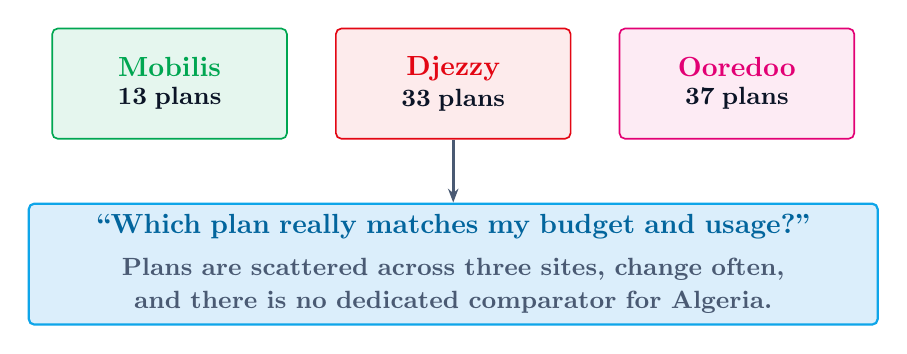
\begin{tikzpicture}[node distance=6mm]
  \node[box, fill=mobilis!10, draw=mobilis, text width=2.7cm, minimum height=1.4cm]
    (m) {\color{mobilis}\bfseries\normalsize Mobilis\\[2pt]\color{ink}\small 13 plans};
  \node[box, fill=djezzy!8, draw=djezzy, text width=2.7cm, minimum height=1.4cm, right=of m]
    (d) {\color{djezzy}\bfseries\normalsize Djezzy\\[2pt]\color{ink}\small 33 plans};
  \node[box, fill=ooredoo!8, draw=ooredoo, text width=2.7cm, minimum height=1.4cm, right=of d]
    (o) {\color{ooredoo}\bfseries\normalsize Ooredoo\\[2pt]\color{ink}\small 37 plans};
  \node[below=8mm of d] (q)
    [abox, text width=10.5cm, minimum height=1.3cm, font=\normalsize]
    {\bfseries ``Which plan really matches my budget and usage?''\\[3pt]
     \color{sec}\small Plans are scattered across three sites, change often, and there is
     no dedicated comparator for Algeria.};
  \draw[fl] (d.south) -- (q.north);
\end{tikzpicture}

\vspace{4pt}
{\color{muted}\footnotesize 83 active plans \textbullet\ \textgreater\,54 million mobile subscribers in Algeria (ARPCE, Q1 2025)}
\end{frame}

% =====================================================================
% 3 — OBJECTIVES
% =====================================================================
\begin{frame}{Objectives}{Five objectives from the FICHE, all delivered}
\centering\small
\renewcommand{\arraystretch}{1.35}
\begin{tabular}{@{}c p{5.4cm} p{5.6cm}@{}}
\toprule
\rowcolor{ink}\color{white}\bfseries \# & \hd{Objective} & \hd{Delivered as} \\
\midrule
1 & Responsive multi-operator comparator & \texttt{/offers} catalogue, filters, 83 live plans \\
2 & Automated data aggregation & Playwright (headless Edge) + Cheerio, daily scrape \\
3 & Intelligent recommendation engine & TOPSIS + rank-order-centroid weights \\
4 & Comparison \& savings visualisation & Side-by-side table, bar charts, savings indicator \\
5 & In-app notification system & Two streams: user (offers) \textbullet\ admin (scrape) \\
\bottomrule
\end{tabular}

\vspace{8pt}
{\color{sec}\footnotesize Method: documentary research (ARPCE, GSMA, DataReportal, Mordor) $\rightarrow$ iterative development, 121 unit tests.}
\end{frame}

% =====================================================================
% 4 — ARCHITECTURE
% =====================================================================
\begin{frame}{System architecture}{Three tiers in one Next.js codebase}
\centering
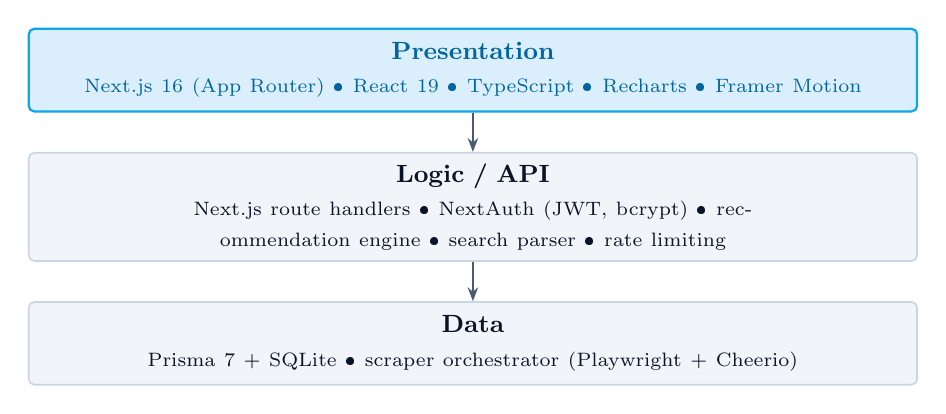
\begin{tikzpicture}[node distance=5mm]
  \node[abox, text width=11cm, minimum height=1.05cm, font=\small] (t1)
    {\bfseries Presentation\\[1pt]\normalfont\scriptsize Next.js 16 (App Router) \textbullet\ React 19 \textbullet\ TypeScript \textbullet\ Recharts \textbullet\ Framer Motion};
  \node[box, text width=11cm, minimum height=1.05cm, font=\small, below=of t1] (t2)
    {\bfseries Logic / API\\[1pt]\normalfont\scriptsize Next.js route handlers \textbullet\ NextAuth (JWT, bcrypt) \textbullet\ recommendation engine \textbullet\ search parser \textbullet\ rate limiting};
  \node[box, text width=11cm, minimum height=1.05cm, font=\small, below=of t2] (t3)
    {\bfseries Data\\[1pt]\normalfont\scriptsize Prisma 7 + SQLite \textbullet\ scraper orchestrator (Playwright + Cheerio)};
  \draw[fl] (t1) -- (t2);  \draw[fl] (t2) -- (t3);
\end{tikzpicture}

\vspace{6pt}
{\color{sec}\footnotesize Full-stack TypeScript — one language across UI and API. SQLite — zero-config, portable, sufficient at this scale.}
\end{frame}

% =====================================================================
% 5 — DATA MODEL
% =====================================================================
\begin{frame}{Data model \textbullet\ class diagram}{Eight domain entities \textbullet\ Prisma schema = single source of truth}
\centering

\includegraphics[height=0.74\textheight]{class_diagram.png}

\vspace{2pt}
{\color{muted}\scriptsize \underline{id} = primary key \quad\textbullet\quad {\color{accentdk}\bfseries field} = foreign key \quad\textbullet\quad NextAuth / infra tables omitted}
\end{frame}

% =====================================================================
% 6 — CONCEPT: WEB SCRAPING
% =====================================================================
\begin{frame}{Concept 1 — Web data aggregation}{Tool: \tool{Playwright (headless Edge) + Cheerio}}
\begin{columns}[T]
\begin{column}{0.5\textwidth}
  {\color{ink}\bfseries\small Why it's the best choice}\\[4pt]
  {\scriptsize
  \renewcommand{\arraystretch}{1.25}
  \begin{tabular}{@{}p{2.2cm} p{4.2cm}@{}}
  \toprule
  \rowcolor{ink}\hd{Option} & \hd{Verdict} \\
  \midrule
  Public API / feed & None published by the operators \\
  Scrapy (no browser) & Blocked by anti-bot \\
  OCR (Tesseract) & 29--43\% confidence — rejected \\
  \rowcolor{accentlt}\color{accentdk}\bfseries Playwright + Cheerio & \color{accentdk}Real browser defeats anti-bot; clean HTML \\
  \bottomrule
  \end{tabular}}\\[6pt]
  {\color{sec}\scriptsize Hierarchy: API \textgreater\ feed \textgreater\ scraping (Boegershausen \& Datta, 2022).}
\end{column}
\begin{column}{0.5\textwidth}
  {\color{ink}\bfseries\small How it works}\\[6pt]
  \centering
  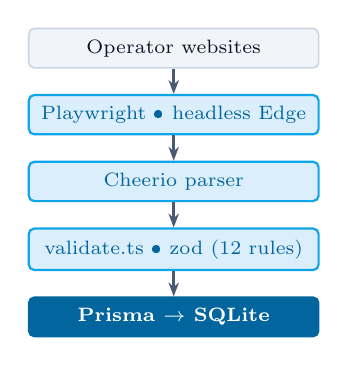
\begin{tikzpicture}[node distance=3.2mm]
    \node[box, text width=3.4cm] (a) {Operator websites};
    \node[abox, text width=3.4cm, below=of a] (b) {Playwright \textbullet\ headless Edge};
    \node[abox, text width=3.4cm, below=of b] (c) {Cheerio parser};
    \node[abox, text width=3.4cm, below=of c] (d) {validate.ts \textbullet\ zod (12 rules)};
    \node[fbox, text width=3.4cm, below=of d] (e) {Prisma $\rightarrow$ SQLite};
    \draw[fl] (a)--(b); \draw[fl] (b)--(c); \draw[fl] (c)--(d); \draw[fl] (d)--(e);
  \end{tikzpicture}
\end{column}
\end{columns}
\vspace{2pt}
{\color{muted}\scriptsize \textbf{Example:} daily cron at 03:00 $\rightarrow$ 83 plans normalised to one schema (MB$\rightarrow$GB, prices, defaults) — catalogue 100\% live.}
\end{frame}

% =====================================================================
% 7 — CONCEPT: RECOMMENDATION (method + why)
% =====================================================================
\begin{frame}{Concept 2 — Recommendation engine}{Tool: \tool{TOPSIS + rank-order-centroid weights}}
\begin{columns}[T]
\begin{column}{0.5\textwidth}
  {\color{ink}\bfseries\small Why it's the best choice}\\[4pt]
  {\scriptsize
  \renewcommand{\arraystretch}{1.25}
  \begin{tabular}{@{}p{2.5cm} p{4.0cm}@{}}
  \toprule
  \rowcolor{ink}\hd{Method} & \hd{Verdict} \\
  \midrule
  Collaborative / ML & No interaction history (cold start) \\
  Weighted sum & Unbounded, scale-sensitive \\
  Lexicographic & Too rigid (ignores trade-offs) \\
  AHP & Too many pairwise comparisons \\
  \rowcolor{accentlt}\color{accentdk}\bfseries TOPSIS + ROC & \color{accentdk}Content-based, bounded score, every step published \\
  \bottomrule
  \end{tabular}}
\end{column}
\begin{column}{0.5\textwidth}
  {\color{ink}\bfseries\small How it works}\\[6pt]
  \centering
  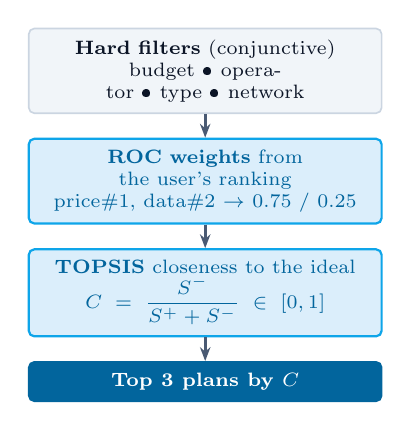
\begin{tikzpicture}[node distance=3mm]
    \node[box, text width=4.2cm] (a) {\textbf{Hard filters} (conjunctive)\\budget \textbullet\ operator \textbullet\ type \textbullet\ network};
    \node[abox, text width=4.2cm, below=of a] (b) {\textbf{ROC weights} from the user's ranking\\ price\#1, data\#2 $\rightarrow$ 0.75 / 0.25};
    \node[abox, text width=4.2cm, below=of b] (c) {\textbf{TOPSIS} closeness to the ideal\\ $C = \dfrac{S^-}{S^+ + S^-}\in[0,1]$};
    \node[fbox, text width=4.2cm, below=of c] (d) {Top 3 plans by $C$};
    \draw[fl] (a)--(b); \draw[fl] (b)--(c); \draw[fl] (c)--(d);
  \end{tikzpicture}
\end{column}
\end{columns}
\vspace{1pt}
{\color{muted}\scriptsize Hwang \& Yoon (1981) \textbullet\ Barron \& Barrett (1996) — nothing in the ranking is invented.}
\end{frame}

% =====================================================================
% 8 — RECOMMENDATION: worked example
% =====================================================================
\begin{frame}{Recommendation — worked example}{Price scored as \emph{value for money} (DA per GB), not raw price}
\centering\small
\renewcommand{\arraystretch}{1.3}
\begin{tabular}{@{}c c c c c@{}}
\toprule
\rowcolor{ink}\hd{Plan} & \hd{Price} & \hd{Data} & \hd{DA / GB} & \hd{} \\
\midrule
A & 600 DA  & 30 GB & \textbf{20}  & \color{ok}\bfseries best value \\
B & 2000 DA & 50 GB & 40           & most data \\
C & 400 DA  & 8 GB  & 80           & cheapest, worst value \\
\bottomrule
\end{tabular}

\vspace{10pt}

\begin{tikzpicture}[node distance=8mm]
  \node[abox, text width=5.2cm, minimum height=1cm] (p)
    {\textbf{Priority = price} $\rightarrow$ \color{ok}\bfseries A \\[2pt]\color{accentdk}\normalfont\scriptsize best value, \emph{not} the cheapest C};
  \node[box, text width=5.2cm, minimum height=1cm, right=18mm of p] (dd)
    {\textbf{Priority = data} $\rightarrow$ \bfseries B\\[2pt]\normalfont\scriptsize the most data};
\end{tikzpicture}

\vspace{6pt}
{\color{muted}\scriptsize The cheapest plan (C) ranks \emph{last} — ``price first'' rewards value for money, not a low sticker price.}
\end{frame}

% =====================================================================
% 9 — CONCEPT: SEARCH
% =====================================================================
\begin{frame}{Concept 3 — Search engine}{Tool: \tool{token parser + SQLite FTS5 (BM25)}}
\begin{columns}[T]
\begin{column}{0.46\textwidth}
  {\color{ink}\bfseries\small Why it's the best choice}\\[4pt]
  {\scriptsize
  \renewcommand{\arraystretch}{1.25}
  \begin{tabular}{@{}p{2.3cm} p{3.6cm}@{}}
  \toprule
  \rowcolor{ink}\hd{Option} & \hd{Verdict} \\
  \midrule
  One big \texttt{LIKE} & Cannot rank, slow \\
  External engine & Extra service, 2nd source of truth \\
  \rowcolor{accentlt}\color{accentdk}\bfseries Parser + FTS5 & \color{accentdk}Exact filters + BM25 relevance, in the DB file \\
  \bottomrule
  \end{tabular}}\\[6pt]
  {\color{sec}\scriptsize FTS5 ships inside SQLite: BM25 ranking, prefix match, accent folding.}
\end{column}
\begin{column}{0.54\textwidth}
  {\color{ink}\bfseries\small How it works}\\[5pt]
  \centering
  \resizebox{\linewidth}{!}{%
  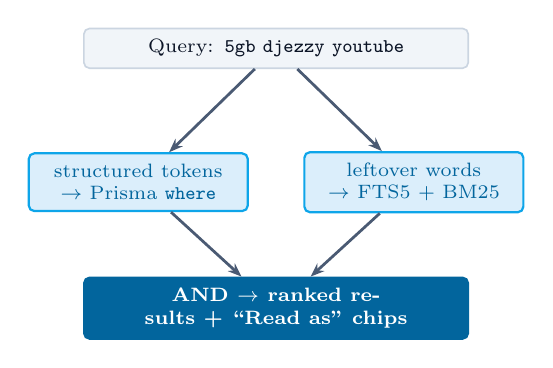
\begin{tikzpicture}
    \node[box, text width=4.6cm] (q) at (0,0) {Query: \texttt{5gb djezzy youtube}};
    \node[abox, text width=2.5cm] (t) at (-1.75,-1.7) {structured tokens\\$\rightarrow$ Prisma \texttt{where}};
    \node[abox, text width=2.5cm] (f) at (1.75,-1.7) {leftover words\\$\rightarrow$ FTS5 + BM25};
    \node[fbox, text width=4.6cm] (r) at (0,-3.3) {AND $\rightarrow$ ranked results + ``Read as'' chips};
    \draw[fl] (q)--(t); \draw[fl] (q)--(f); \draw[fl] (t)--(r); \draw[fl] (f)--(r);
  \end{tikzpicture}}
\end{column}
\end{columns}
\vspace{1pt}
{\color{muted}\scriptsize \textbf{Example:} \texttt{youtube} matches no token $\rightarrow$ FTS5 finds plans whose features mention it; the matched feature is highlighted on the card.}
\end{frame}

% =====================================================================
% 10 — CONCEPT: COMPARISON & VISUALISATION
% =====================================================================
\begin{frame}{Concept 4 — Comparison \& visualisation}{Tool: \tool{comparison table + bar charts (Recharts) + savings}}
\begin{columns}[T]
\begin{column}{0.58\textwidth}
  \centering
  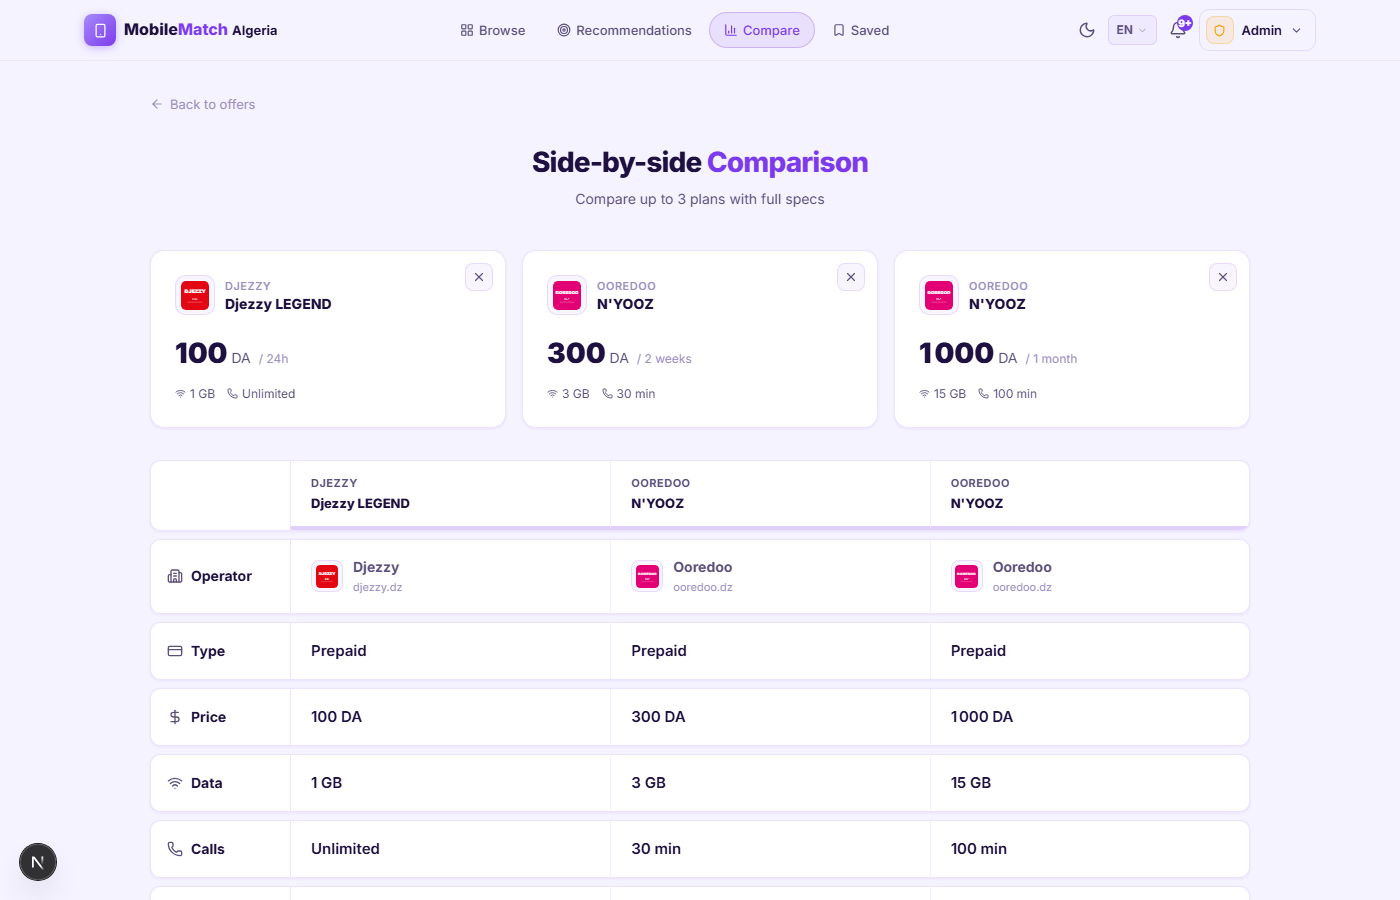
\includegraphics[width=\linewidth]{screenshot_compare.png}
\end{column}
\begin{column}{0.42\textwidth}
  {\color{ink}\bfseries\small Why it's the best choice}\\[5pt]
  \begin{itemize}\setlength\itemsep{4pt}\small
    \item Side-by-side \textbf{table} — the standard pattern for structured products.
    \item \textbf{Bar charts} use position + length, the most accurate visual encoding for quantities (Munzner, 2014).
    \item \textbf{Savings} shown per plan: monthly, annual, \% vs the user's budget.
  \end{itemize}
\end{column}
\end{columns}
\vspace{2pt}
{\color{muted}\scriptsize \textbf{Example:} up to 3 plans, tinted by operator; price / data / annual-savings bar charts.}
\end{frame}

% =====================================================================
% 11 — CONCEPT: NOTIFICATIONS
% =====================================================================
\begin{frame}{Concept 5 — Notification system}{Tool: \tool{publish / subscribe, two separate streams}}
\centering
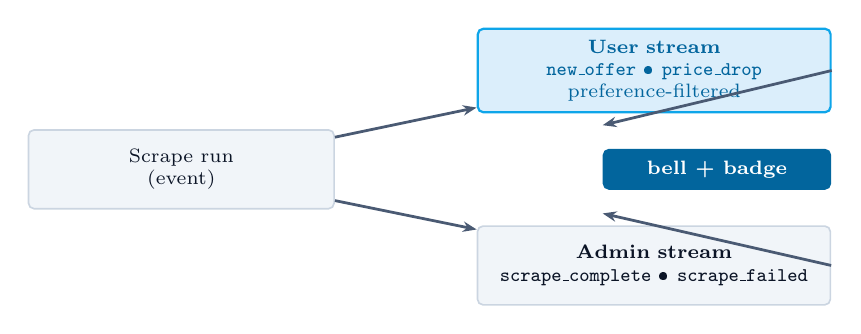
\begin{tikzpicture}[node distance=6mm]
  \node[box, text width=3.6cm, minimum height=1cm] (ev) {Scrape run\\(event)};
  \node[abox, text width=4.2cm, minimum height=1cm, above right=2mm and 18mm of ev] (u)
    {\textbf{User stream}\\\texttt{new\_offer} \textbullet\ \texttt{price\_drop}\\\scriptsize preference-filtered};
  \node[box, text width=4.2cm, minimum height=1cm, below right=2mm and 18mm of ev] (a)
    {\textbf{Admin stream}\\\texttt{scrape\_complete} \textbullet\ \texttt{scrape\_failed}};
  \node[fbox, text width=2.6cm, right=34mm of ev] (bell) {bell + badge};
  \draw[fl] (ev) -- (u); \draw[fl] (ev) -- (a);
  \draw[fl] (u.east) -- ([yshift=3mm]bell.north west);
  \draw[fl] (a.east) -- ([yshift=-3mm]bell.south west);
\end{tikzpicture}

\vspace{8pt}
\begin{columns}[T]
\begin{column}{0.5\textwidth}
  {\color{ink}\bfseries\small Why two streams?}\\[3pt]
  {\color{sec}\scriptsize Each audience sees only what concerns it — a shopper never sees scrape logs, an admin never sees price-drop alerts (publish/subscribe — Eugster et al., 2003).}
\end{column}
\begin{column}{0.5\textwidth}
  {\color{ink}\bfseries\small Why preference-filtered?}\\[3pt]
  {\color{sec}\scriptsize Matching each alert to a declared interest keeps the attention cost low and avoids over-notification (McCrickard \& Chewar, 2003).}
\end{column}
\end{columns}
\end{frame}

% =====================================================================
% 12 — QUALITY & VALIDATION
% =====================================================================
\begin{frame}{Engineering \& validation}{Tested, type-safe, defensible}
\begin{columns}[T]
\begin{column}{0.52\textwidth}
  {\color{ink}\bfseries\small Technology stack}\\[5pt]
  {\scriptsize
  \renewcommand{\arraystretch}{1.3}
  \begin{tabular}{@{}p{2.2cm} p{4.0cm}@{}}
  Next.js 16 & full-stack React framework \\
  Prisma 7 & type-safe ORM, schema = truth \\
  SQLite & zero-config, portable \\
  NextAuth & JWT sessions, bcrypt, roles \\
  Playwright & headless Edge, anti-bot \\
  Vitest & unit + snapshot tests \\
  \end{tabular}}
\end{column}
\begin{column}{0.48\textwidth}
  \centering
  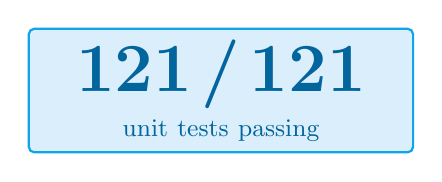
\begin{tikzpicture}
    \node[abox, text width=4.6cm, minimum height=1.5cm, font=\normalsize]
      {\color{accentdk}\fontsize{30}{32}\selectfont\bfseries 121 / 121\\[3pt]\normalfont\small unit tests passing};
  \end{tikzpicture}\\[8pt]
  {\color{sec}\scriptsize Engine \textbullet\ scraping parsers \textbullet\ search parser \textbullet\ helpers.}\\[4pt]
  {\color{sec}\scriptsize + multi-account isolation test: no user can read another's profile, saved list, or notifications.}
\end{column}
\end{columns}
\end{frame}

% =====================================================================
% 13 — LIMITATIONS -> PERSPECTIVES
% =====================================================================
\begin{frame}{Limitations $\rightarrow$ perspectives}{What is honestly missing today, and what closes the gap}
\centering\small
\renewcommand{\arraystretch}{1.3}
\begin{tabular}{@{}p{5.6cm} p{6.0cm}@{}}
\toprule
\rowcolor{ink}\hd{Limitation today} & \hd{Perspective} \\
\midrule
No formal user-survey study & Usability study with external testers (SUS) \\
Scraper fragility on redesigns & Snapshot tests + circuit breaker $\rightarrow$ richer monitoring \\
Image-only plan families excluded & Cloud Vision / LLM extraction \\
Unlimited calls/SMS modelled as binary & Refine to a scoped attribute (on-net vs all) \\
Single-machine evaluation & Public cloud deployment (no code change) \\
\bottomrule
\end{tabular}
\end{frame}

% =====================================================================
% 14 — CONCLUSION
% =====================================================================
\begin{frame}{Conclusion}{}
\centering
\vspace{2pt}
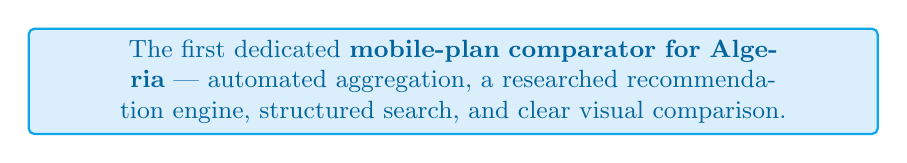
\begin{tikzpicture}[node distance=5mm]
  \node[abox, text width=10.5cm, minimum height=1.0cm, font=\small]
    {The first dedicated \textbf{mobile-plan comparator for Algeria} — automated aggregation,
     a researched recommendation engine, structured search, and clear visual comparison.};
\end{tikzpicture}

\vspace{8pt}
\begin{columns}
\begin{column}{0.33\textwidth}\centering
  {\color{accentdk}\Large\bfseries 83}\\{\color{sec}\footnotesize live plans, 3 operators}\end{column}
\begin{column}{0.33\textwidth}\centering
  {\color{accentdk}\Large\bfseries 5 / 5}\\{\color{sec}\footnotesize objectives delivered}\end{column}
\begin{column}{0.33\textwidth}\centering
  {\color{accentdk}\Large\bfseries 121}\\{\color{sec}\footnotesize tests passing}\end{column}
\end{columns}

\vspace{10pt}
{\color{sec}\footnotesize Every tool choice is backed by the literature; the recommendation ranking uses only published formulas.}
\end{frame}

% =====================================================================
% 15 — THANK YOU
% =====================================================================
{\setbeamertemplate{footline}{}
\begin{frame}[plain]
  \vfill
  \begin{flushleft}\hspace{0.6cm}%
  {\color{accentdk}\bfseries\footnotesize MOBILE MATCH ALGERIA}\\[8pt]
  {\color{ink}\fontsize{46}{50}\selectfont\bfseries Thank you.}\\[8pt]
  {\color{sec}\Large Questions and discussion welcome.}\\[10pt]
  {\color{accent}\rule{1.2cm}{2.5pt}}\\[10pt]
  {\color{ink}\small\bfseries Live demo\;\; http://localhost:3000}\\[3pt]
  {\color{sec}\small Source\;\; github.com/Riad-Amt00/Mobile-Match-Algeria}\\[8pt]
  {\color{muted}\footnotesize AMRATE Riad \textbullet\ IFAG Alger \textbullet\ June 2026}
  \end{flushleft}
  \vfill
\end{frame}}

\end{document}
